\chapter{行波法}
\thispagestyle{empty}

\noindent \dy[行波]{XB}\quad 一往无前向前传播的波
\begin{itemize}
	\item 一维行波\quad 抖动的绳子
	\item 二维行波\quad 投石入海
	\item 三维行波\quad 灯塔上发出的光
\end{itemize}
\noindent \dy[行波法]{XBF}\quad \textbf{无界域内波动方程定解问题的求解方法}

\section{一维波动方程的达朗贝尔公式}
\subsection{达朗贝尔公式的推导}
考虑无界域内波动方程的通解问题
\begin{align}
	\begin{cases}
		\, \dfrac{\partial^2 u}{\partial t^2} = a^2 \dfrac{\partial^2 u}{\partial x^2}, & -\infty < x< +\infty\\[0.5em]
		\, u|_{t = 0} = \varphi(x), & -\infty < x< +\infty\\[0.5em]
		\, \left. \dfrac{\partial u}{\partial t} \right|_{t = 0} = \psi(x) & -\infty < x< +\infty
	\end{cases}
\end{align}

\noindent \textbf{思路}
\begin{itemize}
	\item 仿照\textbf{求解常微分方程的方法}:先求通解,再求特解
	\item 一般来说对偏微分这种方法不可行,但是对于\textbf{一阶波动方程来说是一个特例}
\end{itemize}

\begin{enumerate}[\textbf{步骤}1 ]
	\item 求通解\\
	引入
	\begin{align}
		\begin{cases}
			\, \xi = x + at\\
			\, \eta = x - at
		\end{cases}
	\end{align}
	利用复合函数求导法则,得
	\begin{align*}
		\dfrac{\partial u}{\partial t} = \dfrac{\partial u}{\partial \xi}\dfrac{\partial \xi}{\partial t} + \dfrac{\partial u}{\partial \eta} \dfrac{\partial \eta}{\partial t} = a \dfrac{\partial u}{\partial \xi} - a \dfrac{\partial u}{\partial \eta} = A
	\end{align*}
	\begin{align*}
		\dfrac{\partial^2 u}{\partial t^2} &= \dfrac{\partial A}{\partial t} = a \dfrac{\partial A}{\partial \xi} - a \dfrac{\partial A}{\partial \eta} \\[0.5em]
		&= a\left(a \dfrac{\partial^2 u}{\partial \xi^2} - a \dfrac{\partial }{\partial \eta \partial \xi}\right) - a \left(a \dfrac{\partial^2 u}{\partial \xi \partial  \eta} - a \dfrac{\partial^2 u}{\partial \eta^2}\right)\\[0.5em]
		& = a^2 \left(\dfrac{\partial^2 u}{\partial \xi^2} - 2\dfrac{\partial^2 u}{\partial \xi \partial \eta} + \dfrac{\partial^2 u}{\partial \eta^2}\right)
	\end{align*}
	同理可得
	\begin{align*}
		\dfrac{\partial u}{\partial x} = \dfrac{\partial u}{\partial \xi}\dfrac{\partial \xi}{\partial x} + \dfrac{\partial u}{\partial \eta} \dfrac{\partial \eta}{\partial x} = \dfrac{\partial u}{\partial \xi} + \dfrac{\partial u}{\partial \eta} = B
	\end{align*}
	\begin{align}
		\dfrac{\partial^2 u}{\partial t^2} &= \dfrac{\partial B}{\partial t} = \dfrac{\partial B}{\partial \xi} + \dfrac{\partial B}{\partial \eta} \notag\\[0.5em]
		&= \left(\dfrac{\partial^2 u}{\partial \xi^2} +\dfrac{\partial }{\partial \eta \partial \xi}\right) + \left(\dfrac{\partial^2 u}{\partial \xi \partial  \eta} + \dfrac{\partial^2 u}{\partial \eta^2}\right) \notag\\[0.5em]
		& = \dfrac{\partial^2 u}{\partial \xi^2} + 2\dfrac{\partial^2 u}{\partial \xi \partial \eta} + \dfrac{\partial^2 u}{\partial \eta^2}
	\end{align}
	将以上求偏微分结果代入原方程,可得
	\begin{align}
		\dfrac{\partial^2 u}{\partial \xi \partial \eta} = 0
	\end{align}
	对$\eta$积分得到
	\begin{align*}
		\dfrac{\partial u}{\partial \xi} = f(\xi)
	\end{align*}
	再对$\xi$积分得到
	\begin{align}
		u(x, t) &= \int f(\xi) \, \d \xi + f_2(\eta)\notag \\
		& = f_1(x+at) + f_2(x-at)
	\end{align}

	\item \textbf{用初始条件定特解}\\
	将通解$u(x,t) = f_1(x+at) + f_2(x-at)$代入初始条件
	\begin{align*}
		\begin{cases}
			\, f_1(x) + f_2(x) = \varphi (x)\\
			\, af_1'(x) - af_2'(x) = \psi(x)
		\end{cases}
	\end{align*}
	对导数项积分,可得
	\begin{align*}
		af_1'(x) - af_2'(x) = \psi(x) \quad \Rightarrow \quad af_1(x) - af_2(x) = \int_0^x \psi(\tau) \, \d \tau + C \quad \Rightarrow \quad f_1(x) - f_2(x) = \dfrac{1}{a} \int_0^x \psi(\tau) \, \d \tau + C
	\end{align*}
	即
	\begin{align}
		\begin{cases}
			\, f_1(x) + f_2(x) = \varphi (x)\\[0.5em]
			\, \displaystyle f_1(x) - f_2(x) = \dfrac{1}{a} \int_0^x \psi(\tau) \, \d \tau + C
		\end{cases}
		\quad \Rightarrow \quad
		\begin{cases}
			\,\displaystyle  f_1(x) = \dfrac{\varphi(x)}{2} + \dfrac{1}{2a} \int_0^x \psi(\tau) \, \d \tau + \dfrac{C}{2}\\[1em]
			\, \displaystyle f_2(x) = \dfrac{\varphi(x)}{2} - \dfrac{1}{2a} \int_0^x \psi(\tau) \, \d \tau - \dfrac{C}{2}
		\end{cases}
	\end{align}
	由此可以得到最终解为
	\begin{align}
		u(x,t) = \dfrac{1}{2}\left[\varphi(x+at) + \varphi(x -at)\right] + \dfrac{1}{2a} \int_{x - at}^{x + at}\psi(\tau) \, \d \tau
		\label{达朗贝尔}
	\end{align}
	公式\eqref{达朗贝尔}被称为无限长弦自由振动的\dy[达朗贝尔公式]{DLBEGS}。
\end{enumerate}

\subsection{达朗贝尔公式的物理意义}
\begin{enumerate}[1.]
	\item $\bm{f_1(x + at), f_2(x - at)}$\textbf{的意义}
	\begin{itemize}
		\item $u_2 = f_2(x - at)$的物理意义
		\begin{figure}[!htb]
			\centering
			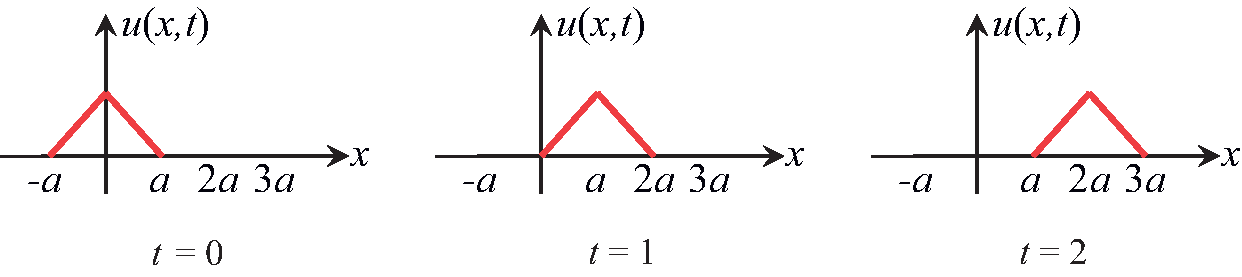
\includegraphics[width=0.7\linewidth]{pic/行波物理意义.pdf}
			\vspace*{-1em}
			\caption{$u_2 = f_2$的物理意义}
			\vspace*{-1em}
			\label{行波物理意义}
		\end{figure}
		\begin{itemize}
			\item 如图\ref{行波物理意义}.随着时间$t$的推移,$u_2$的图形以速度$a$向$x$轴正向移动;
			\item 它表示一个以速度$a$向$x$轴正方向行进的波, 称为\dy[右行波]{YXB}。
		\end{itemize}
		\item $u_1 = f_1(x + at)$的物理意义\\
		\hspace*{2em}同理,$u_1$表示一个以速度$a$向$x$轴负方向行进的波, 称为\dy[左行波]{ZXB}。
	\end{itemize}
	\vspace*{1em}

	\item \textbf{达朗贝尔公式的分析}\\[0.5em]
	令$\varPhi(x) = \dfrac{1}{a} \displaystyle \int_{x_0}^{x} \psi(\tau) \, \d \tau$,则达朗贝尔公式可以写成\vspace*{-0.5em}
	\begin{align}
		u(x,t) &= \dfrac{1}{2}\left[\varphi(x+at) + \varphi(x -at)\right] + \dfrac{1}{2a} \int_{x - at}^{x + at}\psi(\tau) \, \d \tau \notag \\[0.5em]
		& = \dfrac{1}{2}\left[\varphi(x+at) + \varphi(x -at)\right] + \dfrac{1}{2}\left[\varPhi(x+at) - \varPhi(x -at) \right]
	\end{align}
	\begin{itemize}
		\item 第一项表示初位移激发的行波;\\
		\hspace*{2em} $t > 0$以后分成波形相同的两部分,等速向左、向右传播。
		
		\item 第二项表示初速度激发的行波;\\
		\hspace*{2em} $t > 0$以后分成波形相反的两部分,等速向左、向右传播。
	\end{itemize}
	\vspace*{1em}

	\item \textbf{达朗贝尔公式的物理意义}
	\begin{itemize}
		\item 弦上的任意扰动(初位移和初速度)总是以行波的形式分别向两个方向传播出去;
		\item 其传播速度恰恰是波动方程中出现的常数$a$;
		\item 基于这种原因,达朗贝尔解法又称为行波法;
		\item 初位移激发的左右行波是大小相等的,初速度激发的行波与其发生干涉。
	\end{itemize}
\end{enumerate}

\warn[
行波法小总结\vspace*{-0.5em}
{
\begin{enumerate}[\hspace*{2em}1.]
	\item 其要领是引入坐标变换简化方程,求得通解后再求特解;\vspace*{-0.5em}
	\item 一维无界域波动方程的解可以利用达朗贝尔公式直接得到解;\vspace*{-0.5em}
	\item \textbf{仅适用于无界域波动方程的初值问题}。
\end{enumerate}
}
]

\section{特征线}
\begin{enumerate}[1. ]
	\item \textbf{影响区域}
		\begin{itemize}
			\item 0时刻施加在区间$[X_1,X_2]$的扰动在$t$时刻波及$[X_1-at, X_2+at]$。
			\item 梯形区域以外,波动不受区间$[X_1,X_2]$上初始扰动的影响。
			\item 这个不断膨胀的梯形区域称为区间$[X_1, X_2]$的\dy[影响区域]{YXQY}。
		\end{itemize}
	\begin{figure}[!htb]
		\begin{minipage}{0.5\linewidth}
			\centering
			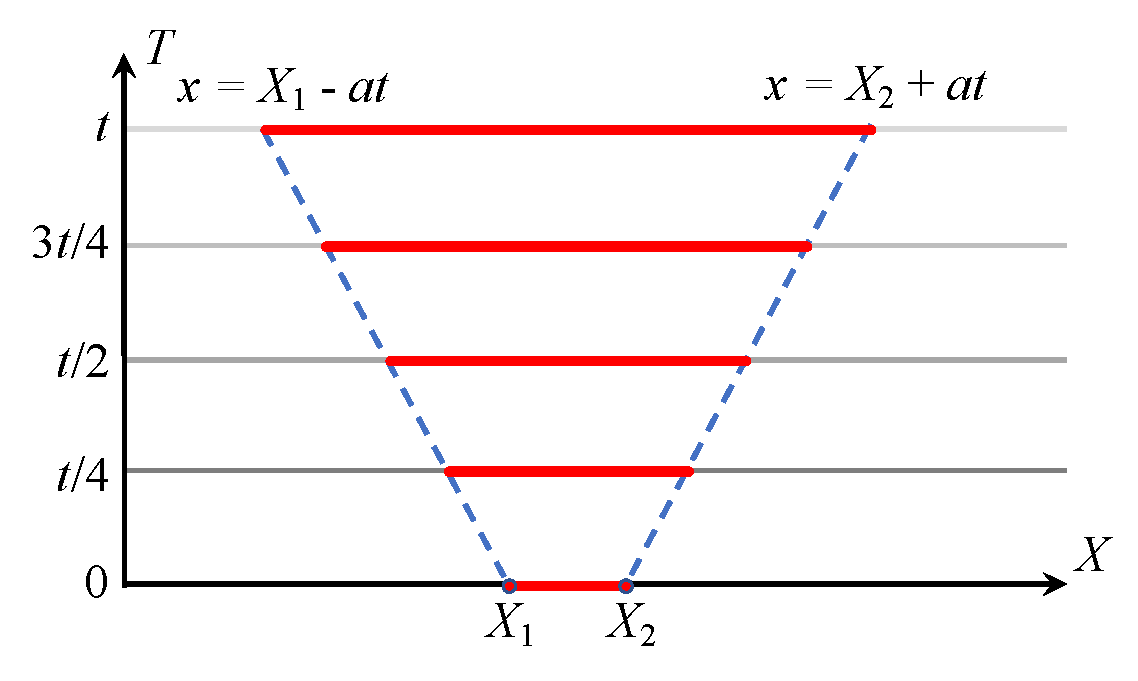
\includegraphics[width=0.9\linewidth]{pic/影响区域.pdf}
			\caption{影响区域}
			\label{影响区域}
		\end{minipage}
		\begin{minipage}{0.5\linewidth}
			\centering
			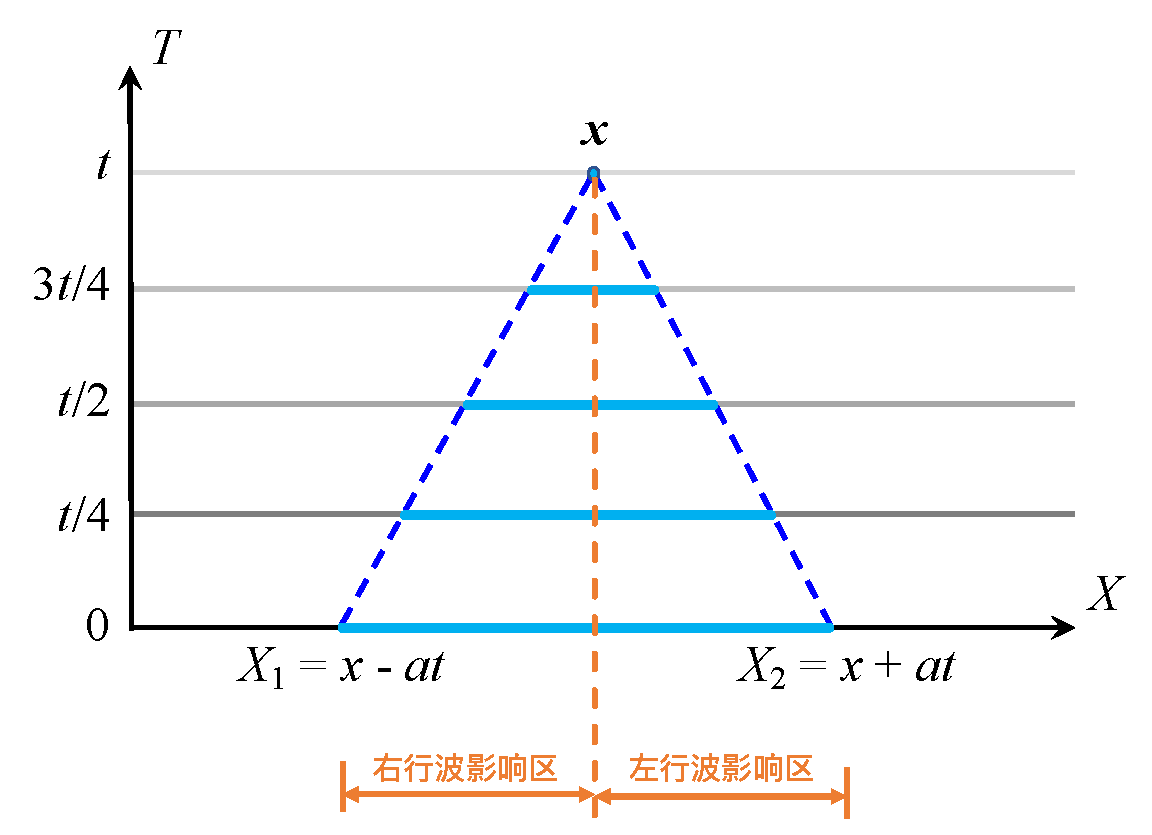
\includegraphics[width=0.85\linewidth]{pic/决定区域.pdf}
			\vspace*{-1.5em}
			\caption{决定区域}
			\label{决定区域}
		\end{minipage}
	\end{figure}
	
	\item \textbf{依赖区间与决定区域}
		\begin{itemize}
			\item $t$时刻$x$点的状况,由区间$[X_1, X_2] = [x-at, x+at]$内的初始条件决定。
			\item 区间$ [x-at, x+at]$称为$(x,t)$的\dy[依赖区间]{YLQJ}。
			\item 对于三角形区域内的任何一点,其\textbf{依赖区间}均位于$ [x-at, x+at]$内部。
			\item 已知$[X_1,X_2]$区间的初始条件,则可以完全确定三角形区域内初值问题的解,这个三角形区域称为区间$[X_1,X_2]$的\dy[决定区域]{JDQY}。
		\end{itemize}
	
		\begin{figure}[!htb]
			\centering
			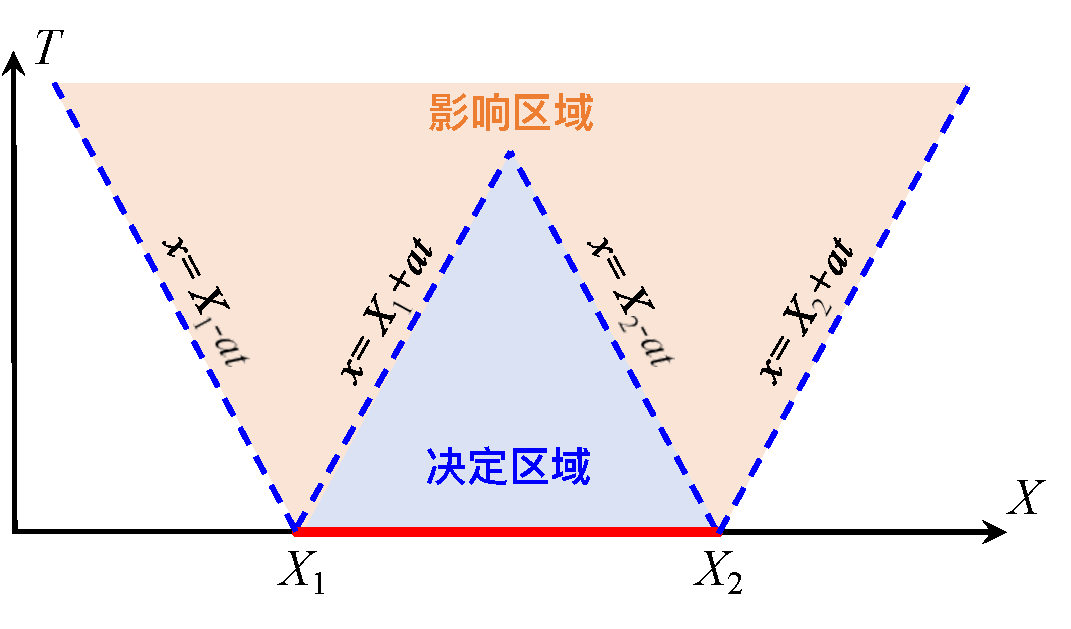
\includegraphics[width=0.55\linewidth]{pic/影响区域和决定区域.pdf}
			\vspace*{-2em}
			\caption{决定区域和影响区域的边界}
			\label{决定区域和影响区域的边界}
		\end{figure}
	
	\item \textbf{决定区域和影响区域的边界}\\
		\hspace*{2em}决定区域和影响区域的边界是由左倾直线$x+at = c_1$和右倾直线$x - at = c_2$规定,这两条直线在$x - t$平面上斜率为$\pm \dfrac{1}{a}$的直线称为一维波动方程的\dy[特征线]{TZX}。
		\begin{itemize}
			\item 在左倾直线$x + at =c_1$上,左行波$f_1(x + at)$的位移为常数。
			\item 在右倾直线$x - at = c_2$上,右行波$f_2(x - at)$的位移为常数。
			\item 所以,左右行波是沿着各自的特征线传播的。
		\end{itemize}
\end{enumerate}


\section{二阶线性双变量偏微分方程}
\begin{enumerate}[1.]
	\item \textbf{特征线的一般化}\\
	\hspace*{2em}对于一般的\dy[二阶线性双变量偏微分方程]{EJXXSBLPWFFC}
	\begin{align}
		A \dfrac{\partial^2 u}{\partial x^2} + 2B\dfrac{\partial^2 u}{\partial x \partial y} + C \dfrac{\partial^2 u}{\partial y^2} + D\dfrac{\partial u}{\partial x} + E \dfrac{\partial u}{\partial y} + Fu = G
	\end{align}
	我们将常微分方程
	\begin{align}
		A(\d y)^2 -2 B \d x \d y + C(\d x)^2 = 0
	\end{align}
	称为相应偏微分方程的\dyn{特征方程},其解为偏微分方程的\dyn{特征线}。特征线的特点:
	\begin{itemize}
		\item 特征线仅与方程中的二阶导数项的系数有关
		\item 利用特征线构造坐标变换,可以实现方程的简化
	\end{itemize}
\vspace*{0.5em}
	
	\item \textbf{二阶线性双变量微分方程的分类}\\
	\hspace*{2em} 对于一般的二阶线性双变量偏微分方程
	\begin{align*}
			A \dfrac{\partial^2 u}{\partial x^2} + 2B\dfrac{\partial^2 u}{\partial x \partial y} + C \dfrac{\partial^2 u}{\partial y^2} + D\dfrac{\partial u}{\partial x} + E \dfrac{\partial u}{\partial y} + Fu = G
	\end{align*}
其判别式与分类如表\ref{二阶线性双变量微分方程的分类}.
	\begin{table}[!htb]
		\centering
		\setlength{\tabcolsep}{12mm}{
			\begin{tabular}{cc}
				\toprule[1.5pt] 
				\multicolumn{2}{c}{判别式 $\Delta  = B^2 - AC$} \\
				\midrule
				$\Delta > 0$ & \dy[双曲线型]{SQXX}的二阶线性双变量微分方程\\
				\hline
				$\Delta = 0$ & \dy[抛物线型]{PWXX}的二阶线性双变量微分方程\\
				\hline
				$\Delta < 0$ & \dy[椭圆型]{TYX}的二阶线性双变量微分方程\\
				\bottomrule[1.5pt]
			\end{tabular}  
		}
		\caption{二阶线性双变量微分方程的分类}
		\label{二阶线性双变量微分方程的分类}
	\end{table} 
	
\end{enumerate}

\section{三维波动方程的泊松公式}
三维波动的定解问题
\begin{equation}
	\begin{cases}
		\, \dfrac{\partial^2 u}{\partial t^2} = a^2 \left(\dfrac{\partial^2 u}{\partial x^2} + \dfrac{\partial^2 u}{\partial y^2} + \dfrac{\partial^2 u}{\partial z^2}\right), & -\infty < x,y,z<+\infty, t>0\\[0.5em]
		\, u\Big|_{t = 0} = \varphi_0 (x,y,z) , & -\infty < x,y,z<+\infty \\[0.7em]
		\, \dfrac{\partial u}{\partial t}\Bigg|_{t = 0} = \varphi_1(x,y,z), & -\infty < x,y,z<+\infty
	\end{cases}
\end{equation}

\subsection{三维波动方程的球对称解}
\noindent \textbf{1. 球坐标系}
	\begin{align}
		\begin{cases}
			\, x = x_0 + r \sin \theta \cos \varphi \\
			\, y = y_0 + r \sin \theta \sin \varphi \\
			\, z = z_0 + r \cos \theta
		\end{cases}
	\end{align}
\noindent \textbf{2. 球对称解}

	引入球坐标系后的三维波动方程转换为
	\begin{align}
		\dfrac{\partial^2 u}{\partial t^2} = a^2 \Bigg[\dfrac{1}{r^2} \dfrac{\partial }{\partial r}\left(r^2 \dfrac{\partial u}{\partial r} \right)+ \dfrac{1}{r^2 \sin \theta} \dfrac{\partial }{\partial \theta} \left(\sin \theta \dfrac{\partial u}{\partial \theta} \right)+ \dfrac{1}{r^2 \sin^2 \theta} \dfrac{\partial^2 u}{\partial \varphi^2}\Bigg]
	\end{align}

	\dy[球对称]{QDC}指的是$u$与$\theta,\rho$无关,只是$r$的函数。此时,波动方程化简为
	\begin{equation}
		\dfrac{\partial^2 u}{\partial t^2} = \dfrac{a^2}{r^2}\dfrac{\partial }{\partial r} \left(r^2 \dfrac{\partial u}{\partial r}\right)
	\end{equation}
	经过等价变形,得到
	\begin{align}
		\dfrac{\partial^2(ru)}{\partial t^2} = a^2 \dfrac{\partial^2(ru)}{\partial r^2}
	\end{align}

	其为关于$ru$的一维波动方程,其通解为
	\begin{equation}
		ru = f_1(r+at) + f_2(r-at)
	\end{equation}

	等价于
	\begin{equation}
		u(r,t) = \dfrac{f_1(r+at) + f_2(r-at)}{r}
	\end{equation}
	其中,$u$可以分为两个部分的叠加
	\begin{itemize}
		\item $\dfrac{f_1(r+at)}{r}$\quad 以速度$a$沿$r$减小的方向传播的行波
		\item $\dfrac{f_2(r-at)}{r}$\quad 以速度$a$沿$r$增加的方向传播的行波
	\end{itemize}


\subsection{三维波动方程的泊松公式}
	三维波动方程在球对称情形下是非常容易求解的,泊松提出了\dy[泊松球面平均法]{PSQMPJF}
	\begin{enumerate}[\hspace*{3em} 1. ]
		\item 考虑空间中以点$M(x,y,z)$为球心,以$r$为半径的球,建立球坐标
		\item 记其球面$M'$上$u$的平均值为$\overline{u}(r,t)$
		\item 对于每一个局部的球心$M$,平均值$\overline{u}(r,t)$满足球对称解
		\item 再求极限$\lim\limits_{r \to 0} \overline{u}(r,t) = u(M, t)$即得到了想要的结果
	\end{enumerate}

\begin{figure}[!htb]
	\centering
	\vspace*{-1em}
	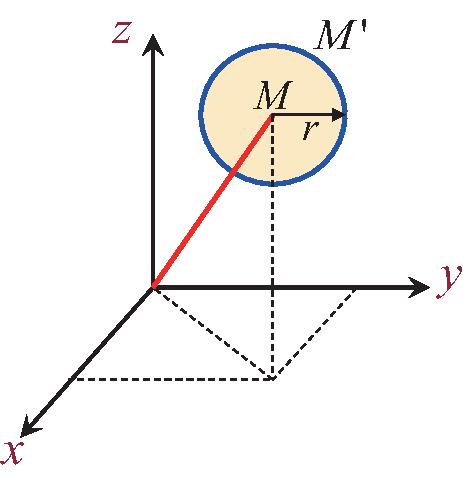
\includegraphics[width=0.25\linewidth]{pic/泊松球面平均法.pdf}
	\vspace*{-1em}
	\caption{泊松球面平均法}
	\label{泊松球面平均法}
\end{figure}

\noindent \textbf{1. 求$\overline{u}(r,t)$的通解}
\begin{enumerate}[\hspace*{2em} (1) ]
	\item 选定球心$M(x,y,z)$,建立球坐标系
	\item 其半径为$r$的球面上的点记作$M’(\xi,\eta,\zeta)$,$(\xi,\eta,\zeta)$是在直角坐标系上的坐标
	\item 对于每一个球心$M$,引入球面平均值函数$\overline{u}(r,t)$
	\begin{equation}
		\overline{u}(r,t) = \dfrac{1}{4 \pi r^2} \iint \limits_{S_{r}^M} u(\xi,\eta,\zeta,t) \, \d S
	\end{equation}
	\textcolor{red}{注意:积分是基于以$M$为原点的球坐标系}
	\item 能够证明其满足球对称解,即其通解为
	\begin{equation}
		r\overline{u}(r, t) = f_1(r+at) + f_2(r- at)
	\end{equation}
\end{enumerate}

\noindent \textbf{2. 求$\overline{u}(r,t)$的特解}
\begin{enumerate}[\hspace*{2em} (1) ]
	\item 由通解得到
	\begin{equation}
		\begin{cases}
			\, r \overline{u}\big|_{t = 0} = f_1(r) + f_2(r)\\[1em]
			\, r \dfrac{\partial \overline{u}}{\partial t}\Bigg|_{t = 0} = af_1'(r) -af_2'(r)
		\end{cases}
	\label{u(r,t)1}
	\end{equation}
	\item 由定解条件可得
	\begin{equation}
		\begin{cases}
			\, \overline{u}\big|_{t = 0} = \varphi_0(x,y,z)\\[1em]
			\, \dfrac{\partial \overline{u}}{\partial t}\Bigg|_{t = 0} = \varphi_1(x,y,z)
		\end{cases} \quad \Longrightarrow \quad \,\,
	\begin{cases}
		\, r \overline{u}\big|_{t = 0} = r\overline{\varphi}_0(r)\\[1em]
		\, r \dfrac{\partial \overline{u}}{\partial t}\Bigg|_{t = 0} = r\overline{\varphi}_1(r)
	\end{cases}
	\label{u(r,t)2}
	\end{equation}
	\item 对比\eqref{u(r,t)1}和\eqref{u(r,t)2}可得
	\begin{equation}
		\begin{cases}
			\,  f_1(r) + f_2(r) = r\overline{\varphi}_0(r)\\[0.5em]
			\, f_1'(r) -f_2'(r) = \dfrac{r}{a}\overline{\varphi}_1(r)
		\end{cases} \quad \Longrightarrow \quad
	\begin{cases}
		\, \displaystyle f_1(r) = \dfrac{1}{2}\Bigg[r\overline{\varphi}_0(r)  + \dfrac{1}{a} \int_0^r \rho \overline{\varphi}_1(\rho) \, \d \rho +C\Bigg]\\[1.2em]
		\, \displaystyle f_2(r) = \dfrac{1}{2}\Bigg[r\overline{\varphi}_0(r)  - \dfrac{1}{a} \int_0^r \rho \overline{\varphi}_1(\rho) \, \d \rho -C\Bigg]
	\end{cases}
	\end{equation}
	\item 反代,得到最终表达式
	\begin{equation}
		\overline{u}(r, t) = \dfrac{1}{2r}\big[(r+at)\overline{\varphi}_0(r+at) + (r-at)\overline{\varphi}_0 (r-at)\big]+ \dfrac{1}{2ar} \int_{r-at}^{r+at}\rho \overline{\varphi}_1(\rho)\, \d \rho 
		\label{u(r,t)}
	\end{equation}
\end{enumerate}

\noindent \textbf{3. 求极限}
\begin{enumerate}[\hspace*{2em} (1) ]
	\item $r \to 0 \Rightarrow M'(\xi, \eta, \zeta) \to M(x,y,z)$
	\item 根据洛必达法则,对\eqref{u(r,t)}分子分母同时求导,并将$r = 0$代入
	\begin{align}
		\lim\limits_{r \to 0} \overline{u}(r,t) & = \lim\limits_{r \to 0 } \dfrac{\big[(r+at)\overline{\varphi}_0(r+at)\big]' + \big[(r-at)\overline{\varphi}_0(r-at)\big]'}{2} + \dfrac{(r + at)\overline{\varphi}_1(r+at)- (r - at)\overline{\varphi}_1(r-at)}{2a}\notag \\[0.5em]
		& = \lim\limits_{r \to 0} \dfrac{\overline{\varphi}_0(r+at)+(r+at)\overline{\varphi}_0'(r+at) + \overline{\varphi}_0(r-at)+ (r-at)\overline{\varphi}_0'(r-at)}{2} + \dfrac{at\overline{\varphi}_1(at)+ at\overline{\varphi}_1(-at)}{2a}\notag \\[0.5em]
		& = \dfrac{\overline{\varphi}_0(at)+at\overline{\varphi}_0'(at) + \overline{\varphi}_0(-at) - at\overline{\varphi}_0'(-at)}{2} + \dfrac{at\overline{\varphi}_1(at)+ at\overline{\varphi}_1(-at)}{2a}\notag \\[0.5em]
		& = \dfrac{\overline{\varphi}_0(at)+\overline{\varphi}_0(-at) + at\overline{\varphi}_0'(at)-at\overline{\varphi}_0'(-at) + t\overline{\varphi}_1(at)+t\overline{\varphi}_1(-at)}{2}
	\end{align}
	\item 可以证明$\overline{\varphi}_0,\overline{\varphi}_1$是偶函数,则$\overline{\varphi}_0',\overline{\varphi}_1'$是奇函数,进一步化简得到
	\begin{equation}
		\begin{cases}
			\, \overline{\varphi}_0(at) = \overline{\varphi}_0(-at)\\
			\, \overline{\varphi}_1(at) = \overline{\varphi}_1(-at)\\
			\, \overline{\varphi}_0'(at) = -\overline{\varphi}_0'(-at)
		\end{cases}
		\quad \Longrightarrow \quad
		\overline{u}(M,t) = \varphi_0(at) + at\overline{\varphi}_0'(at) + t\overline{\varphi}_1(at)
	\end{equation}
	即
	\begin{align}
		\overline{u}(M,t) &= \dfrac{1}{a} \dfrac{\partial }{\partial t} \big[(at)\overline{\varphi}_0(at)\big] + t \overline{\varphi}_1(at) \notag \\[1em]
		& = \dfrac{1}{4 \pi a} \dfrac{\partial }{\partial t}\iint \limits_{S_{at}^M} \dfrac{\varphi_1}{at}\, \d S + \dfrac{1}{4 \pi a} \iint \limits_{S_{at}^M} \dfrac{\varphi_0}{at} 
		\label{三维泊松方程}
	\end{align}
	公式\eqref{三维泊松方程}称为\dy[三维波动方程的泊松公式]{SWBDFCDPSGS}。
\end{enumerate}

\warn[
\textbf{使用三维波动方程的泊松公式的注意事项}
{
\begin{enumerate}
	\item 积分是基于以$M$为原点的球坐标系,所以
	\begin{equation}
		\d S = r^2 \sin \theta \, \d \theta \d \varphi = (at)^2 \sin \theta \, \d \theta \d \varphi
	\end{equation}
	\item 计算时,要将球面$S_{at}^M$上的点变换为以$M$为原点的球坐标系上的点,即\\
	{
		\begin{minipage}{0.4\linewidth}
			\centering
			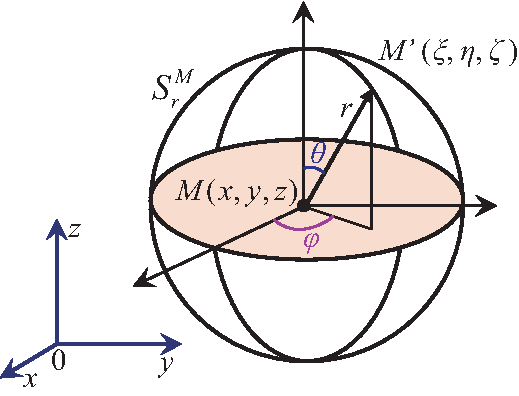
\includegraphics[width=0.75\linewidth]{pic/球坐标系.pdf}
			\vspace*{-1em}
			\captionof{figure}{以$M$为原点的球坐标系}
			\label{球坐标系}
		\end{minipage}
		\begin{minipage}{0.6\linewidth}
			\[
			\varphi_0(x,y,z) \to \varphi_0(\xi, \eta, \zeta)\quad \quad \varphi_1(x,y,z) \to \varphi_1(\xi, \eta, \zeta)
			\]
			其中,
			\begin{equation}
				\begin{cases}
					\, \xi = x + at \sin \theta \cos \varphi,\\
					\, \eta = y + at \sin \theta \sin \varphi,\\
					\, \zeta = z + at \cos \theta.
				\end{cases}
			\end{equation}
		\end{minipage}
	}
\end{enumerate}
}
]

\examples 设已知$\varphi_0(x,y,z) = x + y + z,\, \varphi_1(x,y,z) = 0$,代入泊松方程求解。

\solve 由于$\varphi_1 = 0$,代入泊松公式,求以$M$为原点的球面积分
\[
u(M,t) = \dfrac{1}{4 \pi a} \dfrac{\partial }{\partial t}\iint \limits_{S_{at}^M} \dfrac{\varphi_1}{at}\, \d S + \dfrac{1}{4 \pi a} \iint \limits_{S_{at}^M} \dfrac{\varphi_0}{at} = \dfrac{1}{4 \pi a} \dfrac{\partial }{\partial t}\iint \limits_{S_{at}^M} \dfrac{\varphi_1}{at}\, \d S
\]
其中,球面上的函数值为
\[
\varphi_0(\xi,\eta,\zeta) = x+ at\sin\theta \cos \varphi + y + at\sin \theta \sin \varphi + z + at\cos\theta 
\]
因此,
\[
u(M,t) = \dfrac{1}{4 \pi a} \dfrac{\partial }{\partial t} \int_0^{2\pi} \int_0^\pi \dfrac{x + at \sin \theta \cos \varphi + y + at \sin \theta \sin \varphi + z + at \cos \theta}{at}(at)^2 \sin \theta\, \d \varphi \d \theta = x + y + z
\]
\vspace*{0.5em}

\subsection{三维波动方程泊松公式的物理意义}
\vspace*{0.5em}
\begin{minipage}{0.4\linewidth}
	\centering
	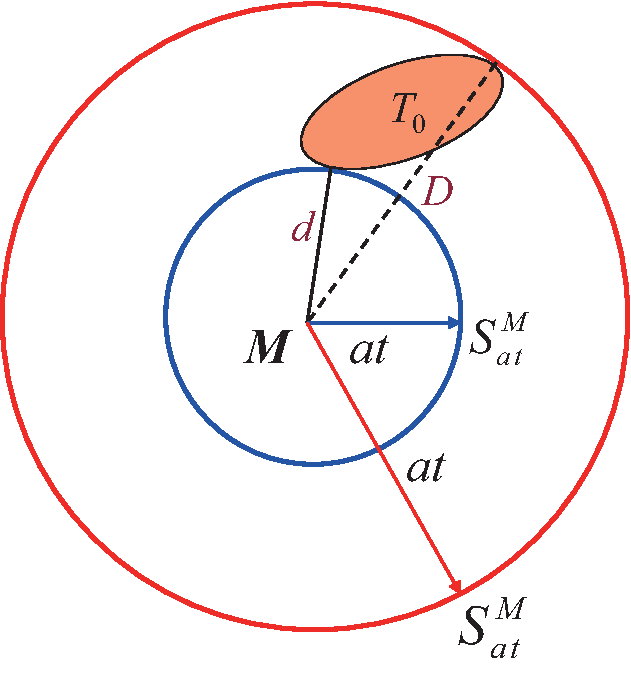
\includegraphics[width=0.7\linewidth]{pic/三维泊松物理意义.pdf}
	\vspace*{-1em}
	\captionof{figure}{三维波动方程泊松公式的物理意义}
	\label{三维波动方程泊松公式的物理意义}
\end{minipage}
\begin{minipage}{0.6\linewidth}
	如图\ref{三维波动方程泊松公式的物理意义},假定初始条件限于立体区域$T_0$
	\begin{itemize}
		\item $at < d\quad \to \quad u(M,t) = 0$\quad 扰动前锋未到
		\item $at > d\quad \to \quad u(M,t) = 0$\quad 扰动阵尾已过
		\item $d \le at \le D \quad \to \quad u(M,t) \neq 0$ \quad 扰动发生作用
		\item 从而可以看出扰动作用有清晰的“前锋”及“阵尾”,它称为\dy[惠更斯原理]{HGSYL}(无\dy[后效现象]{HXXX})。
	\end{itemize}
\end{minipage}
\vspace*{1em}

\subsection{二维波动方程泊松公式及其物理意义}
\noindent \textbf{1. 二维波动方程的泊松公式}

二维波动方程的定解问题为
\begin{equation}
			\begin{cases}
			\, \dfrac{\partial^2 u}{\partial t^2} = a^2 \left(\dfrac{\partial^2 u}{\partial x^2} + \dfrac{\partial^2 u}{\partial y^2} \right), & -\infty < x,y<+\infty, t>0\\[0.7em]
			\, u\Big|_{t = 0} = \varphi_0 (x,y) , & -\infty < x,y<+\infty \\[0.7em]
			\, \dfrac{\partial u}{\partial t}\Bigg|_{t = 0} = \varphi_1(x,y), & -\infty < x,y<+\infty
	\end{cases}
\end{equation}

\dy[二维波动方程的泊松公式]{EWBDFCDPSGS}为
\begin{equation}
	u(M,t) = \dfrac{1}{4 \pi a} \dfrac{\partial }{\partial t} \left(\iint \limits_{\Sigma_{at}^M}\, \d S\right) + \dfrac{1}{4 \pi a} \iint \limits_{\Sigma_{at}^M}\, \d S
\end{equation}
其中,\vspace*{-0.5em}
\begin{itemize}
	\item $u(M,t)$是由以$M$为中心、$at$为半径的圆域$\Sigma_{at}^M$内的初始条件决定的($u$依赖于整个圆域内的初始条件)\vspace*{-0.5em}
	\item \textcolor{red}{注意:决定区域是圆域内而不是圆环上}
\end{itemize}

\noindent \textbf{2. 二维波动方程泊松公式的物理意义}
\vspace*{1em}

\begin{minipage}{0.4\linewidth}
	\centering
	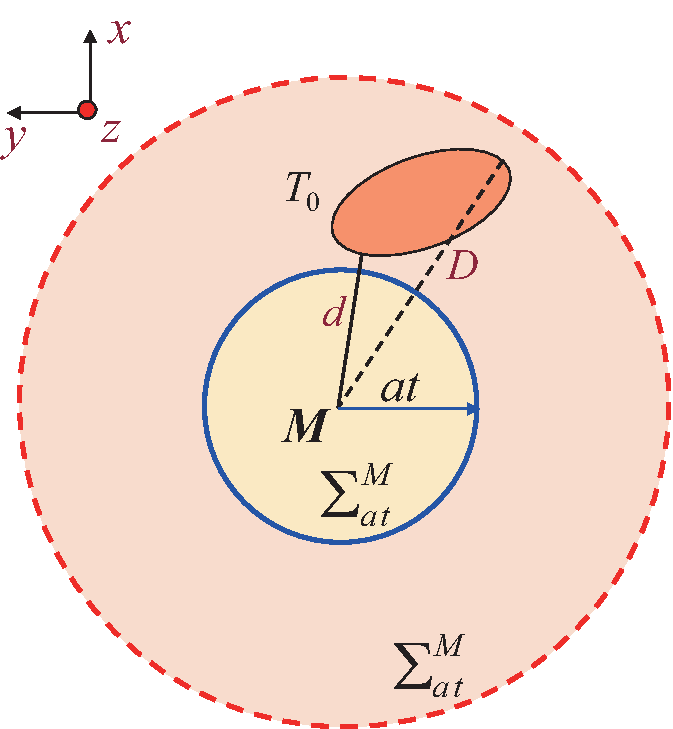
\includegraphics[width=0.7\linewidth]{pic/二维泊松物理意义.pdf}
	\vspace*{-1em}
	\captionof{figure}{二维波动方程泊松公式的物理意义}
	\label{二维波动方程泊松公式的物理意义}
\end{minipage}
\begin{minipage}{0.6\linewidth}
	如图\ref{二维波动方程泊松公式的物理意义},假定初始条件限于平面区域$T_0$
	\begin{itemize}
		\item $at < d\quad \to \quad u(M,t) = 0$\quad 扰动前锋未到
		\item $at \ge d\quad \to \quad u(M,t) \neq 0$\quad 扰动发生作用
		\item 从而可以看出扰动作用有清晰的“前锋”而无“振尾”,称为\dy[波的弥漫]{BDMM}(有后效现象)。
	\end{itemize}
\end{minipage}

\section{泊松公式物理意义总结}
\noindent \textbf{1. 三维泊松公式的物理意义}
\begin{enumerate}[\hspace*{2em} (1) ]
	\item 空间任意一点$M$,在任意时刻$t>0$的状态,完全由以该点为球心、$at$为半径的\textcolor{red}{球面上}初态决定。
	\item 当初始扰动限制在空间某局部范围时,扰动有清晰的“前锋”与“阵尾”,即\textbf{惠更斯原理成立(无后效)}。
\end{enumerate}

\noindent \textbf{2. 二维泊松公式的物理意义}
\begin{enumerate}[\hspace*{2em} (1) ]
	\item 平面任意一点$M$,在任意时刻$t>0$的状态,完全由以该点为圆心、$at$为半径的\textcolor{red}{圆盘域上}初态决定。
	\item 局部初始扰动对二维空间任意一点的扰动有持续后效,波的传播有清晰的“前锋”而无“阵尾”,此现象称为波的弥漫,即\textbf{惠更斯原理不再成立(有后效)}。
\end{enumerate}

















